\begin{tikzpicture}[x=1pt,y=1pt,
    every node/.style={font=\footnotesize},
    ah/.style={draw opacity=0,line width=0.08,fill opacity=1},
    lbl/.style={fill=white,fill opacity=0.88,text opacity=1,
                align=center,inner sep=2.5pt,line width=0.6pt},
    dim/.style={fill=white,align=center,inner sep=2pt,draw=none,font=\scriptsize}]

% ---- Photograph -------------------------------------------------------
\node [anchor=south west,inner sep=0] at (0,0)
  {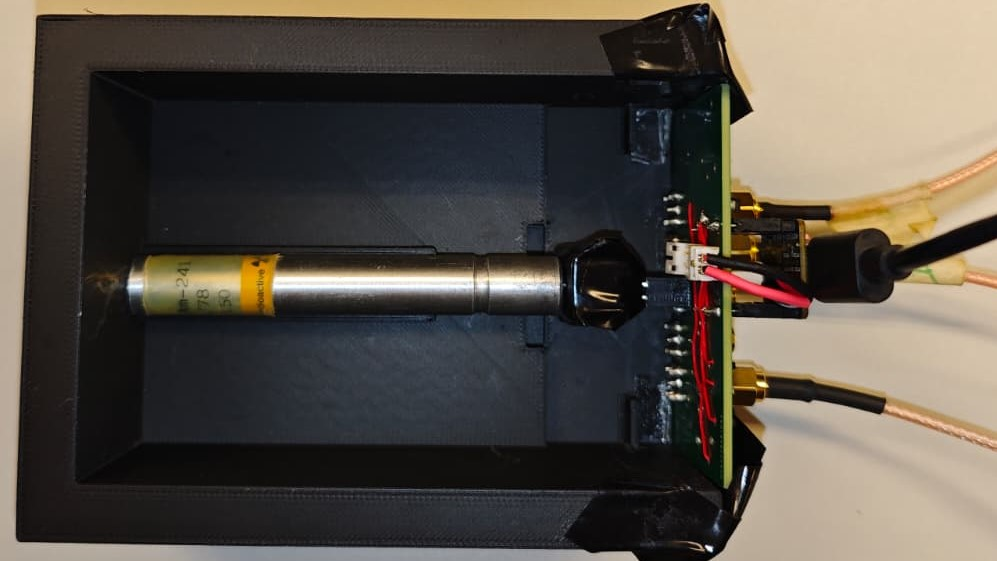
\includegraphics[width=200pt,height=127.1pt]{images/dori_case.jpg}};

% ---- 12 cm dimension (above the image, black) -------------------------
\draw [line width=1.1pt,black] (8.8,134) -- (144.4,134);
\draw [shift={(8.8,134)},rotate=0,ah,fill=black]
      (7.85,-3.78) -- (0,0) -- (7.85,3.78) -- cycle ;
\draw [shift={(144.4,134)},rotate=180,ah,fill=black]
      (7.85,-3.78) -- (0,0) -- (7.85,3.78) -- cycle ;
\node [dim,anchor=center] at (76.6,134) {12~cm};

% ---- Source holder -----------------------------------------------------
\node [anchor=south,align=center,
       text={rgb, 255:red, 204; green, 153; blue, 0 }] at (78,90) {Source Holder};
\draw [color={rgb, 255:red, 204; green, 153; blue, 0 },line width=1.1pt] (62,88) -- (58.15,79.2);
\draw [shift={(55,72)},rotate=66.4,ah,fill={rgb, 255:red, 204; green, 153; blue, 0 }]
      (7.85,-3.78) -- (0,0) -- (7.85,3.78) -- cycle ;
\draw [color={rgb, 255:red, 204; green, 153; blue, 0 },line width=1.1pt] (94,88) -- (100.4,80.5);
\draw [shift={(105.5,74.5)},rotate=130.4,ah,fill={rgb, 255:red, 204; green, 153; blue, 0 }]
      (7.85,-3.78) -- (0,0) -- (7.85,3.78) -- cycle ;

% ---- SiPM + scintillator ----------------------------------------------
\node [lbl,draw={rgb, 255:red, 26; green, 111; blue, 223 },anchor=north east]
      (sipm) at (196,112) {SiPM\\+\\Scintillator};
\draw [color={rgb, 255:red, 26; green, 111; blue, 223 },line width=1.1pt]
      (sipm.west) -| (118.1,77.4);
\draw [shift={(118.1,69.5)},rotate=90,ah,fill={rgb, 255:red, 26; green, 111; blue, 223 }]
      (7.85,-3.78) -- (0,0) -- (7.85,3.78) -- cycle ;

% ---- PCB ---------------------------------------------------------------
\node [lbl,draw={rgb, 255:red, 55; green, 173; blue, 107 },anchor=east]
      (pcb) at (196,49.9) {PCB};
\draw [color={rgb, 255:red, 55; green, 173; blue, 107 },line width=1.1pt]
      (pcb.west) -- (155.4,49.9);
\draw [shift={(147.5,49.9)},rotate=0,ah,fill={rgb, 255:red, 55; green, 173; blue, 107 }]
      (7.85,-3.78) -- (0,0) -- (7.85,3.78) -- cycle ;

% ---- 3D printed test box ----------------------------------------------
\node [lbl,draw={rgb, 255:red, 81; green, 81; blue, 81 },anchor=south east]
      (box) at (196,4) {3D Printed\\Test Box};
\draw [color={rgb, 255:red, 81; green, 81; blue, 81 },line width=1.1pt]
      (box.west) -- (131,15);
\draw [shift={(123,15)},rotate=0,ah,fill=black,
       fill={rgb, 255:red, 81; green, 81; blue, 81 }]
      (7.85,-3.78) -- (0,0) -- (7.85,3.78) -- cycle ;

\end{tikzpicture}